\documentclass{standalone}
\usepackage{tikz}
\usetikzlibrary{circuits.ee.IEC}

\begin{document}

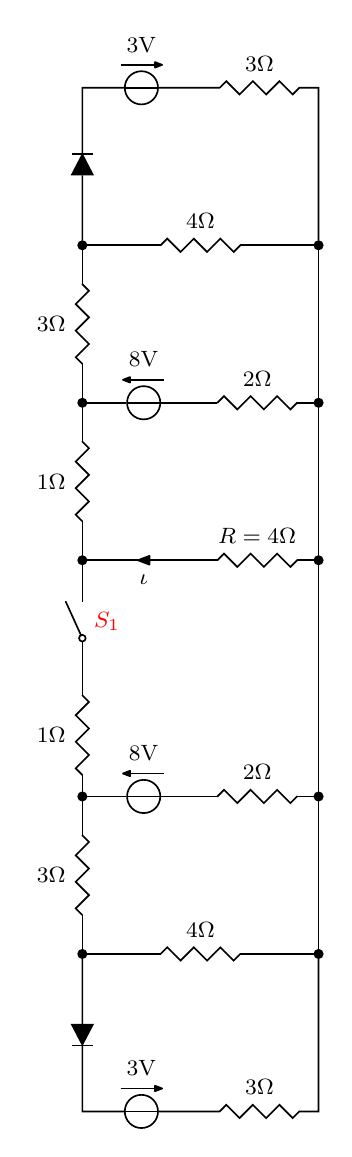
\begin{tikzpicture}[circuit ee IEC, x=3cm, y=2cm, semithick,
                    every info/.style={font=\footnotesize},
                    small circuit symbols,
                    set resistor graphic=var resistor IEC graphic,
                    set diode graphic=var diode IEC graphic,
                    set make contact graphic= var make contact IEC graphic]

  % Define contacts in a loop for easier modification
  \foreach \contact/\y in {1/1, 2/2, 3/3.5, 4/4.5, 5/5.5} {
    \node [contact] (left contact \contact) at (0,\y) {};
    \node [contact] (right contact \contact) at (1,\y) {};
  }

  % Vertical connections
  \draw (right contact 1) -- (right contact 2) -- (right contact 3)
        -- (right contact 4) -- (right contact 5);

  % Circuit components between contacts
  % First row
  \draw (left contact 1) to [diode] ++(down:1)
                         to [voltage source={near start, direction info={volt=3}},
                             resistor={near end, ohm=3}] ++(right:1)
                         to (right contact 1);
  \draw (left contact 1) to [resistor={ohm=4}] (right contact 1);

  % Second row
  \draw (left contact 1) to [resistor={ohm=3}] (left contact 2);
  \draw (left contact 2) to [voltage source={near start, direction info={<-, volt=8}},
                             resistor={ohm=2, near end}] (right contact 2);

  % Third row with switch
  \draw (left contact 2) to [resistor={near start, ohm=1},
                             make contact={near end, info'={[red]$S_1$}}]
                         (left contact 3);
  \draw (left contact 3) to [current direction'={near start, info=$\iota$},
                             resistor={near end, info={$R=4\Omega$}}]
                         (right contact 3);

  % Fourth row
  \draw (left contact 4) to [voltage source={near start, direction info={<-, volt=8}},
                             resistor={ohm=2, near end}] (right contact 4);
  \draw (left contact 3) to [resistor={ohm=1}] (left contact 4);

  % Fifth row
  \draw (left contact 4) to [resistor={ohm=3}] (left contact 5);
  \draw (left contact 5) to [resistor={ohm=4}] (right contact 5);

  % Final row with upward components
  \draw (left contact 5) to [diode] ++(up:1)
                         to [voltage source={near start, direction info={volt=3}},
                             resistor={near end, ohm=3}] ++(right:1)
                         to (right contact 5);

\end{tikzpicture}

\end{document}
